\documentclass[a4paper,12pt,dvipdfm]{article}

\usepackage{sbc-template}
\usepackage{graphicx}
\usepackage{url}
\usepackage[pdftex,raiselinks=false,colorlinks=true,linkcolor=blue,anchorcolor=blue,citecolor=blue,filecolor=blue,urlcolor=blue,linktocpage=true,bookmarksopen=true,pagebackref=true]{hyperref}
\usepackage[latin1]{inputenc}  
\usepackage{listings}
\usepackage{multirow}
\usepackage[brazil]{babel}

\lstset{numbers=left,
stepnumber=1,
firstnumber=1,
numberstyle=\tiny,
extendedchars=true,
breaklines=true,
frame=tb,
basicstyle=\footnotesize,
stringstyle=\ttfamily,
showstringspaces=false
}

\title{Relat�rio sobre An�lise L�xica e Sint�tica de Opera��es de Consulta OCL
- Go}

\author{Alysson Milanez\inst{1}\\ Delano Oliveira\inst{1}\\ Nat� Melo\inst{1}}

\address{
  Departamento de Sistemas e Computa��o\\
  Universidade Federal de Campina Grande (UFCG) -- Campina Grande, PB -- Brasil
  \email{\{alyssonfilgueira, delanohelio, nata.venancio.melo\}@gmail.com}
}

\sloppy

\pagenumbering{arabic}
\begin{document}

\maketitle

\tableofcontents{}
\newpage
\section{Introdu��o}

Neste trabalho iremos apresentar os analisadores l�xico e sint�tico
para Opera��es de Consulta OCL\ldots

\newpage
\section{An�lise L�xica}

O analisador l�xico, l� caracteres da entrada e os agrupa em lexemas,
produzindo um conjunto de tokens e interagindo com a tabela de s�mbolos. Na
an�lise l�xica ocorre a remo��o de espa�os em branco e coment�rios, a correla��o
das mensagens de erros com o programa fonte, o in�cio da constru��o da tabela de
s�mbolos e a expans�o de macros.

\subsection{Ferramenta JFlex}

A ferramenta \textbf{JFlex} gera analisadores l�xicos em \textbf{Java} a partir
da especifica��o de express�es regulares e trechos de c�digo associados a cada
express�o. A especifica��o referida � escrita utilizando a linguaguem JFlex (um
clone da linguagem \textbf{lex}), que tem como extens�o \textbf{.flex}.

\begin{figure}[h] 
	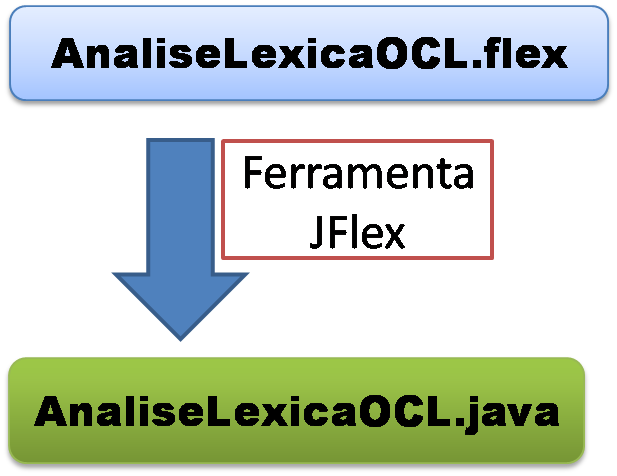
\includegraphics{imagens/analiseLexica.png}
	\caption{(Esquema - ferramenta JFlex.)}
\end{figure}

O esquema acima, ilustra a ferramenta JFlex recebendo como entrada o arquivo
\textbf{AnaliseLexica.flex} e gerando a classe
\textbf{AnaliseLexica.java}. Em linhas gerais, o c�digo gerado l� um arquivo de entrada, extrai cadeias que est�o de acordo com as express�es regulares definidas e executa o c�digo associados as express�es.

\subsection{Linguagem JLex}
	
O arquivo \textbf{AnaliseLexica.flex} � divido em tr�s se��es separadas por
'\%\%'. A primeira se��o serve para incluir c�digo do usu�rio, ou seja, declara��es de imports, classes e m�todos auxiliares, que ser�o copiados diretamente para o topo do arquivo gerado.  A segunda se��o � o espa�o reservado para especificar diretivas, ou seja, declara��es de macros (que definem as express�es regulares) e nomes de estados. Na �ltima se��o s�o definidas as a��es para cada regra especificada anteriormente.

\subsection{Explicitando o arquivo AnaliseLexica.flex}

\scriptsize
\begin{lstlisting}[frame=single, caption={AnaliseLexica.flex}]
package analise_lexica;

import java_cup.runtime.*;
import util.sym; 

%%
%class AnaliseLexica
%unicode
%cup
%line
%column

%{
	StringBuilder string = new StringBuilder();
	
	private Symbol symbol(int tokenname) {
		Symbol symbol = new Symbol(tokenname, yyline, yycolumn, yytext());
		return symbol;
	}
	private Symbol symbol(int tokenname, String value) {
		Symbol symbol = new Symbol(tokenname, yyline, yycolumn, value);
		return symbol;
	}
%}

lineterminator = \n|\r|\n\r|\r\n
inputcharacter = [^\r\n]
whitespace     = {lineterminator}|[ \f\t]
paragraphcomment  = ("/*"~"*/")(~"*/")*
linecomment       = "--" {inputcharacter}* {lineterminator}
comments          = {linecomment} | {paragraphcomment} 

digit  = [0-9] 
letter = [A-Za-z] | [_] 
alpha  = {letter} | {digit} 
identifier = {letter}{alpha}*

%state STRING
stringdelimiter = \'
integer    = -?{digit}+  
real       = {integer}("\."{digit}+)?([eE][+-]?{digit}+)?
boolean = "true"|"false"    
collections = "Set"|"Bag"|"Sequence"|"OrderedSet"|"Collection"

%%

<YYINITIAL>  {whitespace} {  }    
<YYINITIAL>  {comments}   {  }	
<YYINITIAL>  "::"         { return symbol(sym.PATHNAME); } 
<YYINITIAL>  "."          { return symbol(sym.DOT); }
<YYINITIAL>  "->"         { return symbol(sym.COLLECTIONOPERATION); }   
<YYINITIAL>  ":"          { return symbol(sym.COLON); }  
<YYINITIAL>  "("          { return symbol(sym.LEFT_PAR); } 
<YYINITIAL>  "["          { return symbol(sym.LEFT_BRK); } 
<YYINITIAL>  "{"          { return symbol(sym.LEFT_BRA); } 
<YYINITIAL>  ")"          { return symbol(sym.RIGHT_PAR); } 
<YYINITIAL>  "]"          { return symbol(sym.RIGHT_BRK); } 
<YYINITIAL>  "}"          { return symbol(sym.RIGHT_BRA); }   	
<YYINITIAL>  ","          { return symbol(sym.COMMA); } 
<YYINITIAL>  "|"          { return symbol(sym.BAR); }
<YYINITIAL>  "="          { return symbol(sym.EQ); } 
<YYINITIAL>  "<>"         { return symbol(sym.NE); } 
<YYINITIAL>  "<="         { return symbol(sym.LE); } 
<YYINITIAL>  ">="         { return symbol(sym.GE); } 
<YYINITIAL>  "<"          { return symbol(sym.LT); } 
<YYINITIAL>  ">"          { return symbol(sym.GT); } 
<YYINITIAL>  "+"          { return symbol(sym.PLUS); } 
<YYINITIAL>  "-"          { return symbol(sym.MINUS); } 
<YYINITIAL>  "*"          { return symbol(sym.TIMES); } 
<YYINITIAL>  "/"          { return symbol(sym.DIVIDE); } 
<YYINITIAL>  "package"          { return symbol(sym.PACKAGE); }
<YYINITIAL>  "endpackage"       { return symbol(sym.ENDPACKAGE); }
<YYINITIAL>  "context"          { return symbol(sym.CONTEXT); }
<YYINITIAL>  "body"             { return symbol(sym.BODY); }
<YYINITIAL>  "if"               { return symbol(sym.IF); }
<YYINITIAL>  "then"             { return symbol(sym.THEN); }
<YYINITIAL>  "else"             { return symbol(sym.ELSE); }
<YYINITIAL>  "endif"            { return symbol(sym.ENDIF); }
<YYINITIAL>  "implies"          { return symbol(sym.IMPLIES); }
<YYINITIAL>  "and"              { return symbol(sym.AND); }
<YYINITIAL>  "or"               { return symbol(sym.OR); }
<YYINITIAL>  "xor"              { return symbol(sym.XOR); }
<YYINITIAL>  "not"              { return symbol(sym.NOT); }
<YYINITIAL>  "self"              { return symbol(sym.SELF); }
<YYINITIAL>  "String"              { return symbol(sym.STRINGTYPE); }
<YYINITIAL>  "Real"              { return symbol(sym.REALTYPE); }
<YYINITIAL>  "Boolean"              { return symbol(sym.BOOLEANTYPE); }
<YYINITIAL>  "Integer"              { return symbol(sym.INTEGERTYPE); }
<YYINITIAL>  {boolean}          { return symbol(sym.BOOLEAN); }
<YYINITIAL>  {collections}      { return symbol(sym.COLLECTION); }
<YYINITIAL>  {identifier}       { return symbol(sym.IDENTIFIER); } 
<YYINITIAL>  {real}             { return symbol(sym.REAL); } 
<YYINITIAL>  {integer}          { return symbol(sym.INTEGER); }
<YYINITIAL>  {stringdelimiter}  { string.setLength(0); yybegin(STRING); }
<STRING>  [^\n\r\'\\]+          { string.append( yytext()); }
<STRING>  \\t                   { string.append('\t'); }
<STRING>  \\n                   { string.append('\n'); }
<STRING>  \\r                   { string.append('\r'); }
<STRING>  \\\'                  { string.append('\''); }
<STRING>  \\                    { string.append('\\'); }
<STRING> {stringdelimiter} 		{ yybegin(YYINITIAL); return symbol(sym.STRING, string.toString());}

.|\n {throw new Error("Lexema n�o reconhecido pela linguagem OCL: <"+ yytext()+">" + " Linha: "+ (yyline + 1) + " Coluna: "+ (yycolumn + 1)+"\r");}
              
\end{lstlisting}
\normalsize

A seguir ser� explicado o c�digo do arquivo AnaliseLexica.flex.

\subsection{Primeira Se��o}

\subsubsection{Declara��o de pacotes e \textit{imports}}

Na primeira se��o s�o descritos trechos de c�digo java. Na linha 1 � definido o
pacote \verb!analise_lexica!, no qual a classe gerada (em java) ficar�,
nesse caso, a classe gerada ser� AnaliseLexicaOCL.java. Nas linhas 3 e 4 s�o especificados os
\textit{imports} para as classes do pacote \verb!java_cup.runtime.*! e
\textit{sym.java}. Utilizou-se o pacote \verb!analise_lexica! visando organizar
e tornar f�cil a manuten��o das classes java constru�das durante o desenvolvimento do projeto. As classes importadas s�o necess�rias para a manipula��o dos tokens no c�digo gerado.

\subsection{Segunda Se��o}

\subsubsection{Defini��o das op��es a serem usadas}

Nas linhas 7 a 11 s�o descritas as diretivas (opcionais). Na linha 7, define-se
o nome da classe que ser� gerada por meio da diretiva \verb!%class!, nesse caso,
o nome da classe � AnaliseLexica. Na linha 8, usa-se a diretiva \verb!%unicode!,
que define o conjunto de caracteres (UNICODE) que o analisador reconhecer� ao ler um
arquivo textual. Na linha 9, a diretiva \verb!%cup! indica compatibilidade com
o analisador sint�tico CUP. Nas linhas 10 e 11, as diretivas \verb!%line! e
\verb!%column! permitem utilizar as vari�veis \textbf{yyline} e
\textbf{yycolumn}, que armazenam o n�mero da linha e da coluna, respectivamente,
do arquivo que est� sendo lido pelo analisador l�xico.

\subsubsection{Declara��o de vari�veis e m�todos}

Na linha 14, declara-se a vari�vel \textit{string}, do tipo StringBuilder, que
ser� usada para armazenar os caracteres string
encontrados durante a etapa de An�lise L�xica. Das linhas 16 a 19 � especificada a fun��o \textit{symbol}, que ser�
usada para tratar tokens que n�o possuem 'valor-atributo' (e.g. palavras
reservadas da linguagem). Nessa fun��o � criado um objeto Symbol, que armazena
informa��es (nome, linha e coluna onde est� localizado no arquivo) sobre o token
e, em seguida, retornado.

Entre as linhas 20 e 22, a fun��o \textbf{symbol} sofre uma sobrecarga para
lidar com os tokens que possuem o par: \verb!<nome-token, valor-atributo>!. Seu
funcionamento � similar a fun��o \textit{symbol} (definida anteriormente). Esta
fun��es ser�o utilizadas pelo analisador sint�tico.

\subsubsection{Express�es Regulares}

A seguir s�o descritas as express�es regulares utilizadas para definir um
subconjunto da linguagem OCL. Este subconjunto se preocupa com os s�mbolos da linguagem que cobrem a parte de Opera��es de Consulta e os conceitos que est�o ligados a esta parte, como por exemplo, Cole��es, Operadores, dentre outros.

A especifica��o segue com as declara��es de macros. Macros s�o defini��es de
express�es regulares usadas para tornar o c�digo mais f�cil de entender. Uma
declara��o de macro consiste no identificador da macro, seguido do s�mbolo =,
seguido pela express�o regular que a representa: \verb!<nome = defini��o>!. Em
flex, para referenciar uma macro j� criada, basta coloc�-la entre \verb!{ }!.

\subsubsection{Delimitadores de linha}

Nas linhas 26 a 28 s�o declaradas as macros para tratar delimita��o de linha e
espa�o em branco. \textbf{lineterminator}, definida pela express�o
\verb!\n|\r|\n\r|\r\n!, � utilizada para reconhecer os terminadores de linha:
\verb!\n!, \verb!\r! e suas combina��es. \textbf{inputcharacter}, definida pela
express�o regular: \verb![^\r\n]!, reconhece qualquer caractere, exceto os caracteres especiais \verb!\r! e/ou \verb!\n!. \textbf{whitespace}, definida pela express�o \verb!{lineterminator}|[ \f\t]!, reconhece os espa�os em branco, tabula��es e quebras de linha contidas no arquivo fonte do programa que est� sendo analisado.

\subsubsection{Coment�rios}

Os coment�rios em OCL podem ser de dois tipos, conforme a Especifica��o de OCL,
pg. 127. Coment�rios de linha, representados por \verb!--! seguidos por qualquer
sequ�ncia de caracteres que se encontrem na mesma linha, e coment�rios de
par�grafo - representados por \verb!/*! seguido por qualquer cadeia de
caracteres e \verb!*/!, qualquer cadeia delimitada por \verb!/*! e \verb!*/!
ser� desconsiderada pelo analisador l�xico.

Na linha 29 � definida a macro para coment�rio de par�grafo
\textbf{paragraphcomment}, que possui a express�o regular
\verb!("/*"~"*/")(~"*/")*!, indicando que pode existir qualquer cadeia entre
\verb!/*! e \verb!*/!, inclusive eles pr�prios. \verb!("/*"~"*/")! permite que
exista qualquer cadeia entre \verb!/*! e \verb!*/!, exceto \verb!*/!. A
concatena��o com \verb!(~"*/")*! permite incluir a cadeia \verb!*/! dentre as
cadeias que fazem parte do coment�rio.

Na linha 30 � definida a macro para coment�rio de linha \textbf{linecomment},
que consiste em: \verb!"--" {inputcharacter}* {lineterminator}!, um \verb!--!
seguido por qualquer sequ�ncia de caracteres, exceto quebra de linhas.

Na linha 31 � definida a macro para ambos os tipos de coment�rios
\textbf{comments} � qual possui a express�o regular: \verb!{linecomment} | {paragraphcomment}!, indicando que um coment�rio pode ser de linha ou de coluna.

\subsubsection{Alfa num�ricos}

Na linha 33 � definida a macro \textbf{digit} cuja express�o � \verb![0-9]!, que
indica que um d�gito pode ser qualquer valor no intervalo de 0 a 9 (e.g.
\textbf{5} � um \textbf{digit}). 
Na linha 34 � definida a macro para letras ou
sublinhado \textbf{letter}, que possui como express�o regular: \verb![A-Za-z] |[_]!, podendo um \textbf{letter} ser qualquer letra mai�scula, min�scula ou
sublinhado. 
Na linha 35 � definida a macro \textbf{alpha} que consiste numa letra ou
sublinhado ou um digito, e possui express�o: \verb!{letter} | {digit}!.

\subsubsection{Identificadores}

Os identificadores s�o usados para o casamento dos padr�es com os nomes de
fun��es, procedimentos, vari�veis, ou outras express�es que representem
identificadores para as linguagens de programa��o. Em OCL, um identificador deve
ser iniciado com uma letra ou sublinhado e pode ser seguido por qualquer
sequ�ncia de letras, sublinhados ou d�gitos. Desta forma, na linha 36, a macro
\textbf{identifier} � definida com a seguinte express�o:
\verb!{letter}{alpha}*!, garantindo que todos os identificadores reconhecidos na An�lise L�xica iniciar�o com uma letra ou sublinhado e ter� qualquer sequ�ncia de letras, sublinhados ou d�gitos.

\subsubsection{Tipos B�sicos}

A seguir ser�o explicadas as express�es regulares usadas para definir os tipos
b�sicos de OCL \verb!(pg. 74 [KLEPPE])!.

\subsubsection{Tipo String}

Na linha 38 � declarado o estado \verb!STRING!, que ser� usado na parte das
regras l�xicas para auxiliar no reconhecimento de strings. Na linha 39 �
definida a macro \textbf{stringdelimiter}, que � representada pela express�o
\verb!\'!. Serve para reconhecer o delimitador de string, no in�cio e fim, que �
representado por \verb!'!.

\subsubsection{Tipo Integer}

Na linha 40 � definida a  express�o para o tipo Integer \textbf{integer}, com a
express�o: \verb!-?{digit}+!. Iniciando com um \textbf{-} un�rio opcional
seguido pela macro \textbf{digit}, definida anteriormente, a
express�o faz refer�ncia a \textbf{digit} da forma \verb!{digit}!. Em seguida aparece o s�mbol \textbf{+}, indicando que a sequ�ncia anterior n�o pode ser vazia e representando o conjunto de qualquer
sequ�ncia de d�gitos. \textbf{12} � um exemplo do tipo Integer.

\subsubsection{Tipo Real}

Na linha 41 � definida a express�o para o tipo Real \textbf{real}. Baseado na macro \textbf{integer}, definida anteriormente, ela pode
ser subdividida em tr�s subexpress�es para facilitar a explica��o. A express�o inicia com
\verb!{integer}!, indicando que a cadeia come�a com qualquer elemento do
conjunto dos inteiros, seguida por  \verb!("\."{digit}+)?!, indicando que a
cadeia pode ser vazia ou ent�o formada pelo s�mbolo \textbf{.} concatenada por
qualquer elemento do conjunto dos inteiros positivos. Para finalizar, a
subexpress�o \verb!([eE][+-]?{digit}+)?!, indica que o n�mero, representado pela
cadeia \verb!{integer}("\."{digit}+)?!, pode ser ainda ''elevado'' a qualquer
elemento do conjunto dos inteiros positivos \verb!({digit}+)!. O termo
''elevado'' � representado pela cadeia \verb![eE]!, que por sua vez, �
concatenada com a cadeia \verb![+-]?!, indicando se o n�mero ''elevado'' ser�
positivo ou negativo, ou uma cadeia vazia. \textbf{1.23e3} � um exemplo do tipo
Real.

\subsubsection{Tipo Boolean}

Na linha 42 � definida a express�o para o tipo Boolean \textbf{real}
\verb!"true"|"false"!, indicando que o tipo Boolean � formado pelas palavras reservadas \textbf{true} e \textbf{false}.

\subsubsection{Tipos Compostos - Cole��es}

Na linha 43 � definida a express�o \textbf{collections}
\verb!"Set"|"Bag"|"Sequence"|"OrderedSet"!, que representa os tipos de cole��es de OCL, ou seja, as palavras reservadas que
representam cada um dos tipos de cole��es: \textbf{Set, Bag, Sequence e
OrderedSet} \verb!(pg. 137 [KEPLLE])!.

\subsection{Terceira Se��o}

Na terceira se��o s�o descritas as regras das express�es regulares. Todas as
regras seguem o seguinte padr�o: \verb!<estado> express�o { a��o }!. O
analisador l�xico vai lendo a entrada e procurando a sequ�ncia mais longa de caracteres. Caso mais de uma regra case com a sequ�ncia mais longa, escolhe-se aquela que foi definida primeiro. No arquivo AnaliseLexica.flex, na terceira se��o, s�o manipulados dois estados. O estado inicial (YYINITIAL) e o estado que serve para auxiliar no reconhecimento de String (STRING).

Todas as a��es das regras, que aparecem nas linhas 49 a 101, utilizam a fun��o
\textit{symbol} (definada na \textbf{Segunda Se��o}) para retornar o objeto
Symbol (que cont�m as informa��es sobre o token que est� associado a express�o daquela regra). �
passado como argumento para a fun��o \textit{symbol} o nome do token.

\subsubsection{Espa�o e coment�rio}

Nas linhas 47 e 48 s�o tratadas as express�es que reconhecem espa�o em branco e coment�rios, respectivamente. N�o � executada nenhuma a��o para estas duas express�es, ou seja, o analisador est� removendo estas cadeias, que s�o desnecess�rias para realizar o agrupamento dos tokens.

\subsubsection{Nomes de pacotes, opera��o de cole��o, ponto e dois pontos} 

A regra da linha 49 trata o terminal \verb!::!, que no escopo do projeto,
servir� para referenciar tipos em outros pacotes, ou seja, permite navegar nos
pacotes (de UML) at� chegar numa classe desejada. Exemplo: \verb!context NomePacote1::NomePacote2::NomeTipo!.  Na linha 50, a regra trata o s�mbolo
\verb!.!, que no escopo do projeto, � usado para acessar atributos em classes e
permitir executar uma opera��o a partir de um objeto (que n�o seja cole��o).
Exemplo: \verb!Classe1.atributo1.operacao1()!. Na linha 51, a regra trata o
terminal \verb!->!, utilizado para executar opera��es sobre objetos do tipo
Collections. Exemplo: \verb!Bag1->select (...)!. O terminal \verb!:!, associado
a regra da linha 52, � utilizado de diversas formas no escopo deste projeto. As
mais comuns s�o: determinar o in�cio da especifica��o do corpo de uma fun��o
\verb!(body:)!, permitir associar o tipo de Objeto a uma vari�vel no iterador
\textit{forAll}, especificar o tipo de retorno de uma fun��o. Exemplos:
\verb!body: self.atributo, forAll(a : TipoObjeto | express�o)}!.

\subsubsection{Par�nteses, Colchetes, Chaves, V�rgula e Barra}

Os par�nteses, tratados nas regras das linhas 53 e 56, s�o usados em opera��es,
para especificar os argumentos e para determinar a preced�ncia de express�es, em
geral, por exemplo: a express�o \verb!5 - 2 * 10 + 5! resultaria em \verb!-10!,
entretanto, se escrev�ssemos \verb!(5 - 2) * (10 + 5)!, o resultado seria
\verb!45!. Com isso, percebe-se que os par�nteses mudaram a ordem em que foram
realizadas as opera��es. Os colchetes, tratados nas regras das linhas 54 e 57 no
escopo deste projeto, s�o utilizados mais comumente para acessar elementos de
classes compostas por conjunto de outros elementos. Por exemplo, a express�o:
\verb!classeA.conjuntoB[1]! ter� como resultado o primeiro elemento do
\verb!conjuntoB!. 
As chaves, tratadas nas regras das linhas 55 e 58, s�o usadas
para definir cole��es. Por exemplo: \verb!body: Set{1, 2, 3, 4}!. A v�rgula,
tratada na regra da linha 59, � utilizada, no escopo deste projeto, para:
separar os argumentos das opera��es e separar elementos de uma cole��o. A barra,
tratada na regra da linha 60, � utilizada em opera��es, como por exemplo:
\verb!self.employee->exists( p | p.forename = 'Jack' )!.

\subsubsection{Operadores}

Os operadores \verb!=, <>, <=, >=,  <, >, +, -, *, /,! tratados nas regras das
linhas 61 a 70, s�o utilizados para realizar opera��es em valores do tipo
Integer e Real. Os operadores \verb!= e <>! tamb�m s�o utilizados em opera��es
que envolvem valores do tipo String e do tipo Boolean.

\subsubsection{Keywords}

As palavras chaves da linguagem OCL necess�rias para o escopo do projeto s�o:
\textbf{self} (denotar a inst�ncia do contexto), \textbf{package} (especificar
explicitamente a que pacote as express�es pertencem), \textbf{endpackage}
(delimita o ''fim do package''), \textbf{context} (especificar o contexto para
as express�es) e \textbf{body} (definir o corpo da opera��o) e s�o tratadas nas
regras das linhas 71 a 74 e na linha 84 (self). \verb!(pg. 13 e 14 [Especifica��o OCL])!


\subsubsection{Express�o Condicional if-then-else}

As regras das linhas 75 a 78 tratam os elementos que formam a express�o
condicional \verb!''if-then-else''!, s�o eles:  \textbf{if, then, else, endif}. 
\verb!(pg. 10 [Especifica��o OCL])!. Um exemplo de uma express�o condicional
\textbf{if-then-else}:  \verb!if balance > 5000 then 2 else 3 endif!.

\subsubsection{Operadores ''Booleanos''}

As regras das linhas 79 a 83 tratam os operadores ''booleanos'' (al�m dos j�
comentados acima), s�o eles: \textbf{implies, and, or, xor e not} \verb!(pg. 123 [KEPLLE])!. Exemplo: \verb!forAll(elem | self->includes(elem) xor
s->includes(elem))!.

 \subsubsection{Nomes dos Tipos B�sicos}
 
 As regas das linhas 85 a 88 tratam os nomes dos tipos String, Boolean,
 Real e Integer, utilizados para reconhecimento dos nomes dos tipos b�sicos de
 OCL e cria��o de tokens para eles.
 
 \subsubsection{Tipos b�sicos e identificador}
 
As regas das linhas 89 , 90, 92 e 93 tratam os tipos Boolean, Collection, Real e
Integer, respectivamente, baseados nas macros definidas anteriormente, na
\textbf{Segunda Se��o}. Na linha 93, a regra trata a macro que define os
Identificadores (tamb�m explicada na \textbf{Segunda Se��o}). Para auxiliar no
reconhecimento dos valores do tipo String, foi necess�rio criar o estado STRING.
Quando o analisador l�xico encontra um delimitador de String (tratado na linha
94), um poss�vel valor do tipo String poder� ser encontrado, das linhas 95 a
101, os caracteres que podem ser encontrados em Strings s�o tratados.


\newpage
\section{An�lise Sint�tica}
\newpage
\section{Conclus�o}

Nessa etapa do projeto constru�mos o analisador l�xico e sint�tico do nosso
compilador, usamos o JFlex para o analisador l�xico e o JCup para o analisador sint�tico. Com isso foram gerados classes Java (.java) que representam esses dois analisadores.
O desenvolvimento do projeto nos proporcionou colocar em pr�tica toda a teoria
que vimos em sala de aula, desde a especifica��o das express�es regulares
utilizada para cria��o dos tokens, at� a redu��o da Gram�tica OCL (defini��o
da gram�tica do nosso projeto) por meio da defini��o de regras de produ��o, os
terminais e n�o terminais da nossa gram�tica. Ao nos depararmos com a gram�tica
OCL pudemos perceber problemas de ambiguidade, de forma que foi preciso
recorrermos aos conhecimentos que adquirimos em aula para resolvermos tais problemas e podermos chegar � nossa gram�tica livre de
ambiguidade.
A grande vantagem do desenvolvimento de um projeto �, conforme dito acima,
termos a oportunidade de aplicarmos os conceitos vistos.

\newpage
\section{Bibliografia}

\begin{itemize}
  
  \item Ramalho, Franklin. Notas de Aula. Dispon�vel em:
  http://www.dsc.ufcg.edu.br/~franklin/disciplinas/2011-
  1/Compiladores/index.php/Main/PlanoDeAula\\Acesso em: 04 abr. 2011.
  
\end{itemize}
\newpage
\section{Anexo A - Arquivo AnaliseLexica.flex}
\scriptsize
\begin{lstlisting}[frame=single, caption={AnaliseLexica.flex}]
package analise_lexica;

import java_cup.runtime.*;
import util.sym; 

%%
%class AnaliseLexica
%unicode
%cup
%line
%column

%{
	StringBuilder string = new StringBuilder();
	
	private Symbol symbol(int tokenname) {
		Symbol symbol = new Symbol(tokenname, yyline, yycolumn, yytext());
		return symbol;
	}
	private Symbol symbol(int tokenname, String value) {
		Symbol symbol = new Symbol(tokenname, yyline, yycolumn, value);
		return symbol;
	}
%}

lineterminator = \n|\r|\n\r|\r\n
inputcharacter = [^\r\n]
whitespace     = {lineterminator}|[ \f\t]
paragraphcomment  = ("/*"~"*/")(~"*/")*
linecomment       = "--" {inputcharacter}* {lineterminator}
comments          = {linecomment} | {paragraphcomment} 

digit  = [0-9] 
letter = [A-Za-z] | [_] 
alpha  = {letter} | {digit} 
identifier = {letter}{alpha}*

%state STRING
stringdelimiter = \'
integer    = -?{digit}+  
real       = {integer}("\."{digit}+)?([eE][+-]?{digit}+)?
boolean = "true"|"false"    
collections = "Set"|"Bag"|"Sequence"|"OrderedSet"|"Collection"

%%

<YYINITIAL>  {whitespace} {  }    
<YYINITIAL>  {comments}   {  }	
<YYINITIAL>  "::"         { return symbol(sym.PATHNAME); } 
<YYINITIAL>  "."          { return symbol(sym.DOT); }
<YYINITIAL>  "->"         { return symbol(sym.COLLECTIONOPERATION); }   
<YYINITIAL>  ":"          { return symbol(sym.COLON); }  
<YYINITIAL>  "("          { return symbol(sym.LEFT_PAR); } 
<YYINITIAL>  "["          { return symbol(sym.LEFT_BRK); } 
<YYINITIAL>  "{"          { return symbol(sym.LEFT_BRA); } 
<YYINITIAL>  ")"          { return symbol(sym.RIGHT_PAR); } 
<YYINITIAL>  "]"          { return symbol(sym.RIGHT_BRK); } 
<YYINITIAL>  "}"          { return symbol(sym.RIGHT_BRA); }   	
<YYINITIAL>  ","          { return symbol(sym.COMMA); } 
<YYINITIAL>  "|"          { return symbol(sym.BAR); }
<YYINITIAL>  "="          { return symbol(sym.EQ); } 
<YYINITIAL>  "<>"         { return symbol(sym.NE); } 
<YYINITIAL>  "<="         { return symbol(sym.LE); } 
<YYINITIAL>  ">="         { return symbol(sym.GE); } 
<YYINITIAL>  "<"          { return symbol(sym.LT); } 
<YYINITIAL>  ">"          { return symbol(sym.GT); } 
<YYINITIAL>  "+"          { return symbol(sym.PLUS); } 
<YYINITIAL>  "-"          { return symbol(sym.MINUS); } 
<YYINITIAL>  "*"          { return symbol(sym.TIMES); } 
<YYINITIAL>  "/"          { return symbol(sym.DIVIDE); } 
<YYINITIAL>  "package"          { return symbol(sym.PACKAGE); }
<YYINITIAL>  "endpackage"       { return symbol(sym.ENDPACKAGE); }
<YYINITIAL>  "context"          { return symbol(sym.CONTEXT); }
<YYINITIAL>  "body"             { return symbol(sym.BODY); }
<YYINITIAL>  "if"               { return symbol(sym.IF); }
<YYINITIAL>  "then"             { return symbol(sym.THEN); }
<YYINITIAL>  "else"             { return symbol(sym.ELSE); }
<YYINITIAL>  "endif"            { return symbol(sym.ENDIF); }
<YYINITIAL>  "implies"          { return symbol(sym.IMPLIES); }
<YYINITIAL>  "and"              { return symbol(sym.AND); }
<YYINITIAL>  "or"               { return symbol(sym.OR); }
<YYINITIAL>  "xor"              { return symbol(sym.XOR); }
<YYINITIAL>  "not"              { return symbol(sym.NOT); }
<YYINITIAL>  "self"              { return symbol(sym.SELF); }
<YYINITIAL>  "String"              { return symbol(sym.STRINGTYPE); }
<YYINITIAL>  "Real"              { return symbol(sym.REALTYPE); }
<YYINITIAL>  "Boolean"              { return symbol(sym.BOOLEANTYPE); }
<YYINITIAL>  "Integer"              { return symbol(sym.INTEGERTYPE); }
<YYINITIAL>  {boolean}          { return symbol(sym.BOOLEAN); }
<YYINITIAL>  {collections}      { return symbol(sym.COLLECTION); }
<YYINITIAL>  {identifier}       { return symbol(sym.IDENTIFIER); } 
<YYINITIAL>  {real}             { return symbol(sym.REAL); } 
<YYINITIAL>  {integer}          { return symbol(sym.INTEGER); }
<YYINITIAL>  {stringdelimiter}  { string.setLength(0); yybegin(STRING); }
<STRING>  [^\n\r\'\\]+          { string.append( yytext()); }
<STRING>  \\t                   { string.append('\t'); }
<STRING>  \\n                   { string.append('\n'); }
<STRING>  \\r                   { string.append('\r'); }
<STRING>  \\\'                  { string.append('\''); }
<STRING>  \\                    { string.append('\\'); }
<STRING> {stringdelimiter} 		{ yybegin(YYINITIAL); return symbol(sym.STRING, string.toString());}
.|\n {throw new Error("Lexema n�o reconhecido pela linguagem OCL: <"+ yytext()+">" + " Linha: "+ (yyline + 1) + " Coluna: "+ (yycolumn + 1)+"\r");}
              
\end{lstlisting}
\normalsize
\newpage
\section{Anexo B - Arquivo AnaliseSintatica.cup}
\scriptsize
\begin{lstlisting}[frame=single, caption={AnaliseLexica.flex}]
package analise_sintatica;
import java_cup.runtime.Symbol;
import util.Util;

parser code {:
	
	public void report_error(String message, Object info) {
		Util.report_error(message, info);
	}
	public void syntax_error(Symbol cur_token) {
		Util.syntax_error(cur_token);
	}
	public void debug_message(String mess) {
		Util.debug_message(mess);
	}
	public void debug_shift(Symbol shift_tkn) {
		Util.debug_shift(shift_tkn);
	}
	public void debug_reduce(int prod_num, int nt_num, int rhs_size) {
		Util.debug_reduce(prod_num, nt_num, rhs_size);
	}
:};

terminal PACKAGE, ENDPACKAGE, CONTEXT, BODY, COLLECTION, SELF;
terminal DOT, COMMA, COLON, PATHNAME, LEFT_PAR, LEFT_BRK, LEFT_BRA, RIGHT_PAR, RIGHT_BRK, RIGHT_BRA, BAR;
terminal COLLECTIONOPERATION;
terminal EQ, NE, LE, GE, GT, LT;
terminal AND, OR, NOT, XOR, IMPLIES;
terminal IF, ELSE, THEN, ENDIF;
terminal PLUS, MINUS, TIMES, DIVIDE;
terminal INTEGERTYPE, REALTYPE, BOOLEANTYPE, STRINGTYPE;
terminal Integer INTEGER;
terminal Double REAL;
terminal String STRING;
terminal IDENTIFIER, BOOLEAN;

non terminal packageDeclaration;
non terminal packageDeclarationAux;
non terminal contextDeclaration;
non terminal bodyDeclaration;
non terminal operation;
non terminal operationParAux;
non terminal oclExpression;
non terminal parameters;
non terminal pathName;
non terminal pathNameAux;
non terminal pathNameOperation;
non terminal collectionTypeIdentifier;
non terminal ifExp;
non terminal collectionType;
non terminal typeName;
non terminal variableDeclaration;
non terminal relationalExpression;
non terminal relationalExpressionAux;
non terminal additiveExpression;
non terminal additiveExpressionAux;
non terminal multiplicativeExpression;
non terminal multiplicativeExpressionAux;
non terminal postfixExpression;
non terminal postfixExpressionAux;
non terminal operationCall;
non terminal propertyCall;
non terminal propertyCallParameters;
non terminal declarator;
non terminal declaratorAux;
non terminal literalCollection;
non terminal expressionParameter;
non terminal expressionParameterAux;
non terminal qualifiers;
non terminal primaryExpression;
non terminal unaryExpression;
non terminal oclExpressionAux;
non terminal unaryOperator;
non terminal multiplyOperator; 
non terminal addOperator;
non terminal relationalOperator;
non terminal logicalOperator;
non terminal literal;
non terminal primaryTypes;
non terminal colonPathName;
 
precedence left COMMA;
precedence left IMPLIES;
precedence left AND, OR, XOR;
precedence left EQ, NE;
precedence left LE, GE, GT, LT; 
precedence left IF, THEN, ELSE, ENDIF;
precedence left PLUS, MINUS;
precedence left TIMES, DIVIDE;
precedence left NOT;
precedence left LEFT_PAR, RIGHT_PAR;
precedence left COLLECTIONOPERATION, DOT; 

start with packageDeclaration;

packageDeclaration ::=  PACKAGE pathName packageDeclarationAux ENDPACKAGE
		| packageDeclarationAux;
packageDeclarationAux ::= contextDeclaration packageDeclarationAux |;
pathName ::= IDENTIFIER pathNameAux;
pathNameAux ::= PATHNAME pathName |;
pathNameOperation ::= PATHNAME pathName;
contextDeclaration ::= CONTEXT operation bodyDeclaration;
bodyDeclaration ::= BODY IDENTIFIER COLON oclExpression
		| BODY COLON oclExpression;
operation ::= IDENTIFIER pathNameOperation LEFT_PAR operationParAux RIGHT_PAR COLON typeName;
operationParAux ::= parameters |;
parameters ::= variableDeclaration
		| variableDeclaration COMMA parameters;

collectionType ::= collectionTypeIdentifier LEFT_PAR typeName RIGHT_PAR;
collectionTypeIdentifier ::= COLLECTION;
			 
typeName ::= primaryTypes 
		| pathName
		| collectionType;

primaryTypes ::= STRINGTYPE
		| REALTYPE
		| BOOLEANTYPE
		| INTEGERTYPE;
			
literal ::= REAL | INTEGER | BOOLEAN | STRING;
			
variableDeclaration ::= IDENTIFIER COLON typeName;
oclExpression ::= relationalExpression oclExpressionAux;
oclExpressionAux ::= logicalOperator relationalExpression oclExpressionAux |;

relationalExpression ::= additiveExpression relationalExpressionAux;
relationalExpressionAux ::= relationalOperator additiveExpression relationalExpressionAux |;

additiveExpression ::= multiplicativeExpression additiveExpressionAux;
additiveExpressionAux ::= addOperator multiplicativeExpression additiveExpressionAux |;

multiplicativeExpression ::= unaryExpression multiplicativeExpressionAux;
multiplicativeExpressionAux ::= multiplyOperator unaryExpression multiplicativeExpressionAux |;

unaryExpression ::= unaryOperator postfixExpression
					| postfixExpression;

postfixExpression ::= primaryExpression postfixExpressionAux;
postfixExpressionAux ::= operationCall propertyCall postfixExpressionAux |;
operationCall ::= COLLECTIONOPERATION 
		| DOT;
				  
primaryExpression ::= literalCollection
		| literal
		| propertyCall
		| LEFT_PAR oclExpression RIGHT_PAR
		| SELF
		| ifExp;

literalCollection ::= collectionTypeIdentifier LEFT_BRA expressionParameter RIGHT_BRA;
 
ifExp ::= IF oclExpression THEN oclExpression ELSE oclExpression ENDIF;

propertyCall ::= pathName qualifiers propertyCallParameters;

qualifiers ::= LEFT_BRK expressionParameter RIGHT_BRK|;

propertyCallParameters ::= LEFT_PAR expressionParameter RIGHT_PAR
		|LEFT_PAR IDENTIFIER expressionParameterAux RIGHT_PAR
		|LEFT_PAR declarator expressionParameter RIGHT_PAR
		|;
						   
declarator ::= IDENTIFIER declaratorAux colonPathName  BAR oclExpression;
declaratorAux ::= COMMA IDENTIFIER declaratorAux|;
colonPathName ::= COLON pathName |;

expressionParameter ::= oclExpression expressionParameterAux |;
expressionParameterAux ::= COMMA oclExpression expressionParameterAux |;

logicalOperator ::= AND | OR | XOR | IMPLIES;
relationalOperator ::= EQ | NE | LE | GE | GT | LT;
addOperator ::= PLUS | MINUS;
multiplyOperator ::= TIMES | DIVIDE;
unaryOperator ::= MINUS | NOT;
\end{lstlisting}
\normalsize
\end{document}